\section{Installing Docker}

PLEASE READ THIS SECTION CAREFULLY. The installation process is easy, but there are multiple versions of Docker and you have to be careful to install the right one.

\subsection{macOS}

If you have the M1 Mac (Apple silicon), then follow the instructions for the preview build for the M1 here: \url{https://docs.docker.com/docker-for-mac/apple-silicon/}. Note that support for Docker on Apple silicon is still experimental, and we have had issues in the past. If you run into strange issues during normal operation, please let the TAs know.

Otherwise, if your Mac is a 2010 model or newer and is running macOS El Capitan 10.11 or newer, you can head over to Docker’s website at the following link and follow the instructions to install the Community Edition of Docker: \url{https://docs.docker.com/docker-for-mac/install/}

If your Mac is older than 2010, come to office hours or ask on Piazza and we can discuss a solution.

\subsection{Windows}

The distribution of Docker on Windows has recently switched from the legacy ``Docker Toolbox'' to the new ``Docker Desktop for Windows''. To find out which one you should install, you first have to check your Windows version. Open your Start Menu in the bottom left, enter ``\texttt{winver}'', and press enter. \textbf{Note that if you are on Windows 10, you probably want to install the more recent version.}

\begin{itemize}
    \item If the menu indicates that you have Windows Home, and your version is 1903 or above, then see Section \ref{windows-new} below.
    \item If the menu indicates that you have Windows Pro, Enterprise, or Education, and your build number is 16299 or above, then see Section \ref{windows-new} below.
    \item Otherwise, follow Section \ref{windows-old} below.
\end{itemize}

\subsubsection{Windows (Recent)}\label{windows-new}

First, install Git for Windows if you do not already have it, which can be found at the following link:
\url{https://gitforwindows.org/}. In particular, this contains Git Bash, which can be used as a terminal for running bash scripts and other Unix commands on Windows.

The Git installation will prompt you for lots of configuration options about Git; if you don't know what an option means, select the default option.

Next, install Docker Desktop for Windows.

\begin{itemize}
    \item If you found that you have Windows Home, then follow the installation instructions here: \url{https://docs.docker.com/docker-for-windows/install-windows-home/}.
    Additionally, you must install WSL 2. Instructions to do so can be found here: \href{https://docs.microsoft.com/en-us/windows/wsl/install-win10#step-1---enable-the-windows-subsystem-for-linux}{https://docs.microsoft.com/en-us/windows/wsl/install-win10}.

    \item If you found that you have Windows Pro, Enterprise, or Education, then follow the installation instructions here: \url{https://docs.docker.com/docker-for-windows/install/}
\end{itemize}

If prompted to choose between ``Edge'' and ``Stable'' versions to download, select ``Stable''. If prompted to install the necessary components for WSL2, select yes.

Follow the guides up through ``Start Docker Desktop''. You do not need to follow the onboarding tutorial after starting Docker. If you see an error that ``WSL 2 is not installed'', follow the instructions given in Section \ref{windows-new-starting}. Make sure you reboot your computer after installation before proceeding.

\subsubsection{Windows (Legacy)}\label{windows-old}

Firstly, check that you actually want to do this. Unless you are still on Windows 8, this is probably not the option you want.

First, install the latest version of VirtualBox, which can be found at the following link.
\url{https://www.virtualbox.org/wiki/Downloads}, Click on \texttt{Windows Host} to download, then run the installer.

Second, install Docker Toolbox. You can find instructions archived here:
\url{https://web.archive.org/web/20200919160751/https://docs.docker.com/toolbox/toolbox_install_windows/}. The download link will no longer work; you can download Docker Toolbox from the release on GitHub here: \url{https://github.com/docker/toolbox/releases/download/v19.03.1/DockerToolbox-19.03.1.exe}.

\textbf{IMPORTANT:} When installing Docker Toolbox, make sure to uncheck VirtualBox, as shown in the following picture:

\begin{center}
    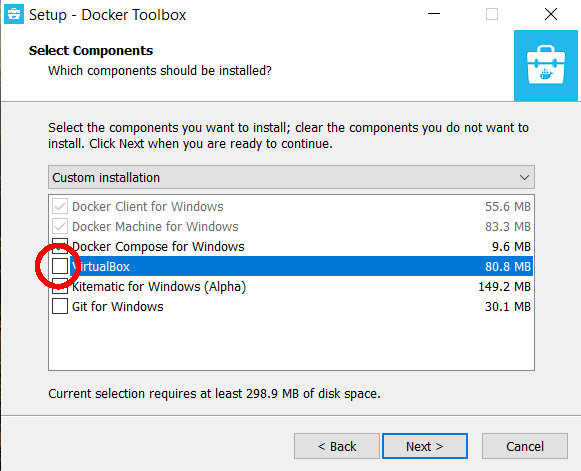
\includegraphics[scale=0.5]{VBOX.png}
\end{center}

\subsection{Linux}
In order to install Docker on Linux (specifically Ubuntu), you need to be running at least Ubuntu 16.04. If you are running a different flavor of Linux, you should be able to find instructions online on how to install it. If you are running Ubuntu 16.04 or newer, follow the instructions here: \url{https://docs.docker.com/install/linux/docker-ce/ubuntu/}. For other Linux distributions, you can follow online instructions; if you get stuck, you can ask a TA or ask for help on Piazza.



\section{CS 2110 Docker Image}
We have created a Docker image for the students of CS 2110 that contains all of the tools that they will need throughout this course. The image itself is hosted on Docker Hub (https://hub.docker.com/r/gtcs2110/cs2110docker/), but we have developed a script for you to use so you don’t need to worry about that. The image is setup to be a very basic Ubuntu 20.04 machine (currently on 18.04 due to technical issues, but will be upgraded soon) that includes the following tools that you need for this class:

\begin{itemize}
  \item CircuitSim (for circuits)
  \item complx (for assembly)
  \item gcc/gdb (for C)
\end{itemize}

One thing that it does not include is a text editor. \textbf{STUDENTS SHOULD NOT EDIT ANY FILES INSIDE OF THE CONTAINER!} When you write code later in the semester, you will edit the files in your favorite text editor \emph{outside} of the container.





\section{Starting up the Docker Image}
Once you have installed Docker, you are ready to download and run the CS 2110 Docker image. To do that, download the \textbf{cs2110docker.sh} script from \texttt{Files $\rightarrow$ Docker Resources} on Canvas, and save it in the directory that you plan on putting all of your code for this class in. Next, we need to make sure Docker is up and running so we can run the script.

\subsection{macOS}
If Docker is running, you will see a little whale on your menu bar in the top right corner of your screen. If it isn’t, go into your Applications folder and double click on the Docker icon to launch it. Click on the whale in the menu bar and wait for the status to say ``Docker is running.'' Once its running, you need to give proper permissions to the the cs2110docker script. Open a terminal window, \texttt{cd} into the directory where you put the script, and run the following:

\begin{center}
    \begin{verbatim}
        sudo chmod +x cs2110docker.sh
    \end{verbatim}
\end{center}

Once you’ve set the permissions (which you only have to do on the first run), you can run the script using the following command:

\begin{center}
    \begin{verbatim}
        ./cs2110docker.sh
    \end{verbatim}
\end{center}

This may take a moment if it is your first time running the script, but if everything goes as planned, you should see eventually see the message ``\texttt{Successfully launched CS 2110 Docker container.}''

\subsection{Windows}

\subsubsection{Windows (Recent)} \label{windows-new-starting}

Make sure you rebooted your computer after installation. The installation process should install a ``Docker Desktop'' application on your computer. Search for this via your Start Menu, and open it.

The first time you open this, it may warn you that ``WSL 2 is not installed''. If this occurs, follow the instructions here to install WSL2: \href{https://docs.microsoft.com/en-us/windows/wsl/install-win10#step-1---enable-the-windows-subsystem-for-linux}{https://docs.microsoft.com/en-us/windows/wsl/install-win10}. You do not need to install a Linux distribution; only follow Step 1 through Step 5.

When the whale in the bottom left of this window is green and says ``Running'' on hover, Docker is ready to run. If you cannot get Docker for Windows to run, you likely have not enabled virtualization in your BIOS---ask a TA for help.

After Docker is started, open Git Bash (open Start Menu and search for ``Git Bash''), use \texttt{cd} to navigate to the directory in which you put the \texttt{cs2110docker.sh} script, and run

\begin{center}
    \begin{verbatim}
        ./cs2110docker.sh
    \end{verbatim}
\end{center}

\textbf{IMPORTANT:} On Windows, place the \texttt{cs2110docker.sh} script somewhere under your home directory, e.g. \texttt{C:\textbackslash{}Users\textbackslash{}gburdell\textbackslash{}...}. In Git Bash, this will appear as \texttt{/c/Users/gburdell/...}, or you may see a ``\texttt{$\sim$}'' as an abbreviation for your home directory.

This may take a moment if it is your first time running the script, but if everything goes as planned, you should see eventually see the message ``\texttt{Successfully launched CS 2110 Docker container.}''

\subsubsection{Windows (Legacy)}

The installation process put an icon on your desktop for Docker Quickstart:

\begin{center}
    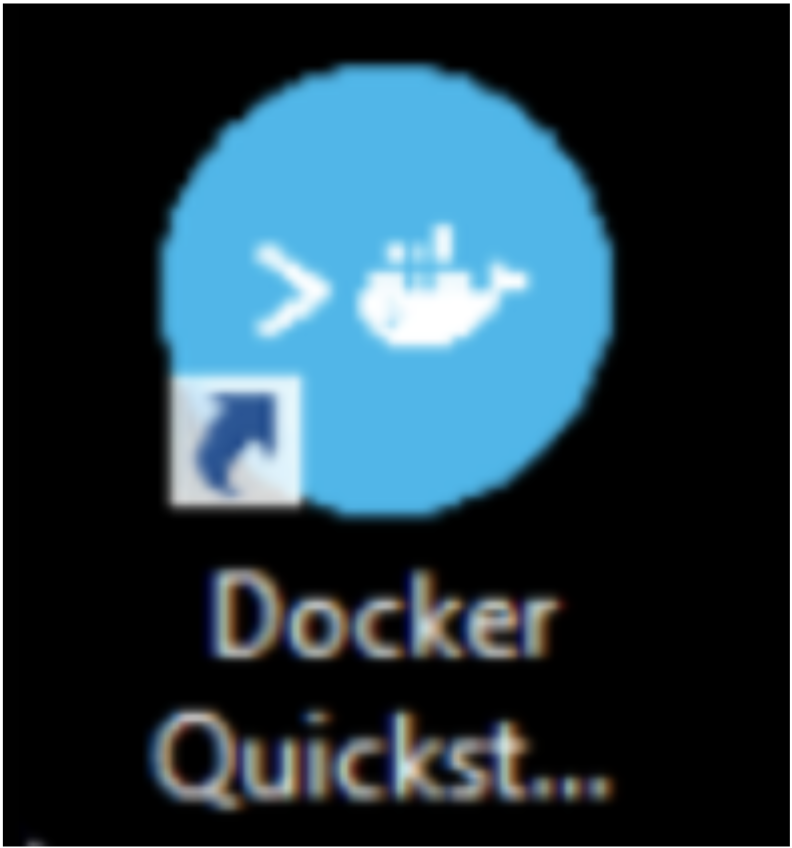
\includegraphics[scale=0.1]{dockerquickstart.png}
\end{center}

Double click on this icon to launch the Docker terminal. From this terminal window, cd into the directory where you put the cs2110docker.sh script. Once you’re there, run it using the following command:

\begin{center}
    \begin{verbatim}
        ./cs2110docker.sh
    \end{verbatim}
\end{center}

\textbf{IMPORTANT:} On Windows, place the \texttt{cs2110docker.sh} script somewhere under your home directory, e.g. \texttt{C:\textbackslash{}Users\textbackslash{}gburdell\textbackslash{}...}. In Git Bash, this will appear as \texttt{/c/Users/gburdell/...}, or you may see a ``\texttt{$\sim$}'' as an abbreviation for your home directory.

This may take a moment if it is your first time running the script, but if everything goes as planned, you should see eventually see the message ``\texttt{Successfully launched CS 2110 Docker container.}''

\subsection{Linux}
If you are running Linux, the installation process should have set the Docker daemon to start on boot, so you don’t need to worry about launching it manually. Before you can run the script, you have to set up the user group for Docker. Open a terminal window and run the following commands:

\begin{center}
    \begin{verbatim}
        sudo groupadd docker
        sudo usermod -aG docker $USER
    \end{verbatim}
\end{center}

Once you’ve created the user group (which you only have to do on the first run), you can run the script using the following command:

\begin{center}
    \begin{verbatim}
        ./cs2110docker.sh
    \end{verbatim}
\end{center}

This may take a moment if it is your first time running the script, but if everything goes as planned, you should see eventually see the message ``\texttt{Successfully launched CS 2110 Docker container.}''


\section{Using the CS 2110 Docker Container}
There are two ways to run the Docker image---using a browser or using a VNC client. When you ran the cs2110docker.sh script, the last line outputted a URL, which should be something along the lines of

\begin{center}
    \begin{verbatim}
        http://<ip-address>:6901/vnc.html
    \end{verbatim}
\end{center}

This URL gives you access to the container from a web browser, which is the easiest way to use it. Open up your browser and go to the URL. You should see this page:
\begin{center}
    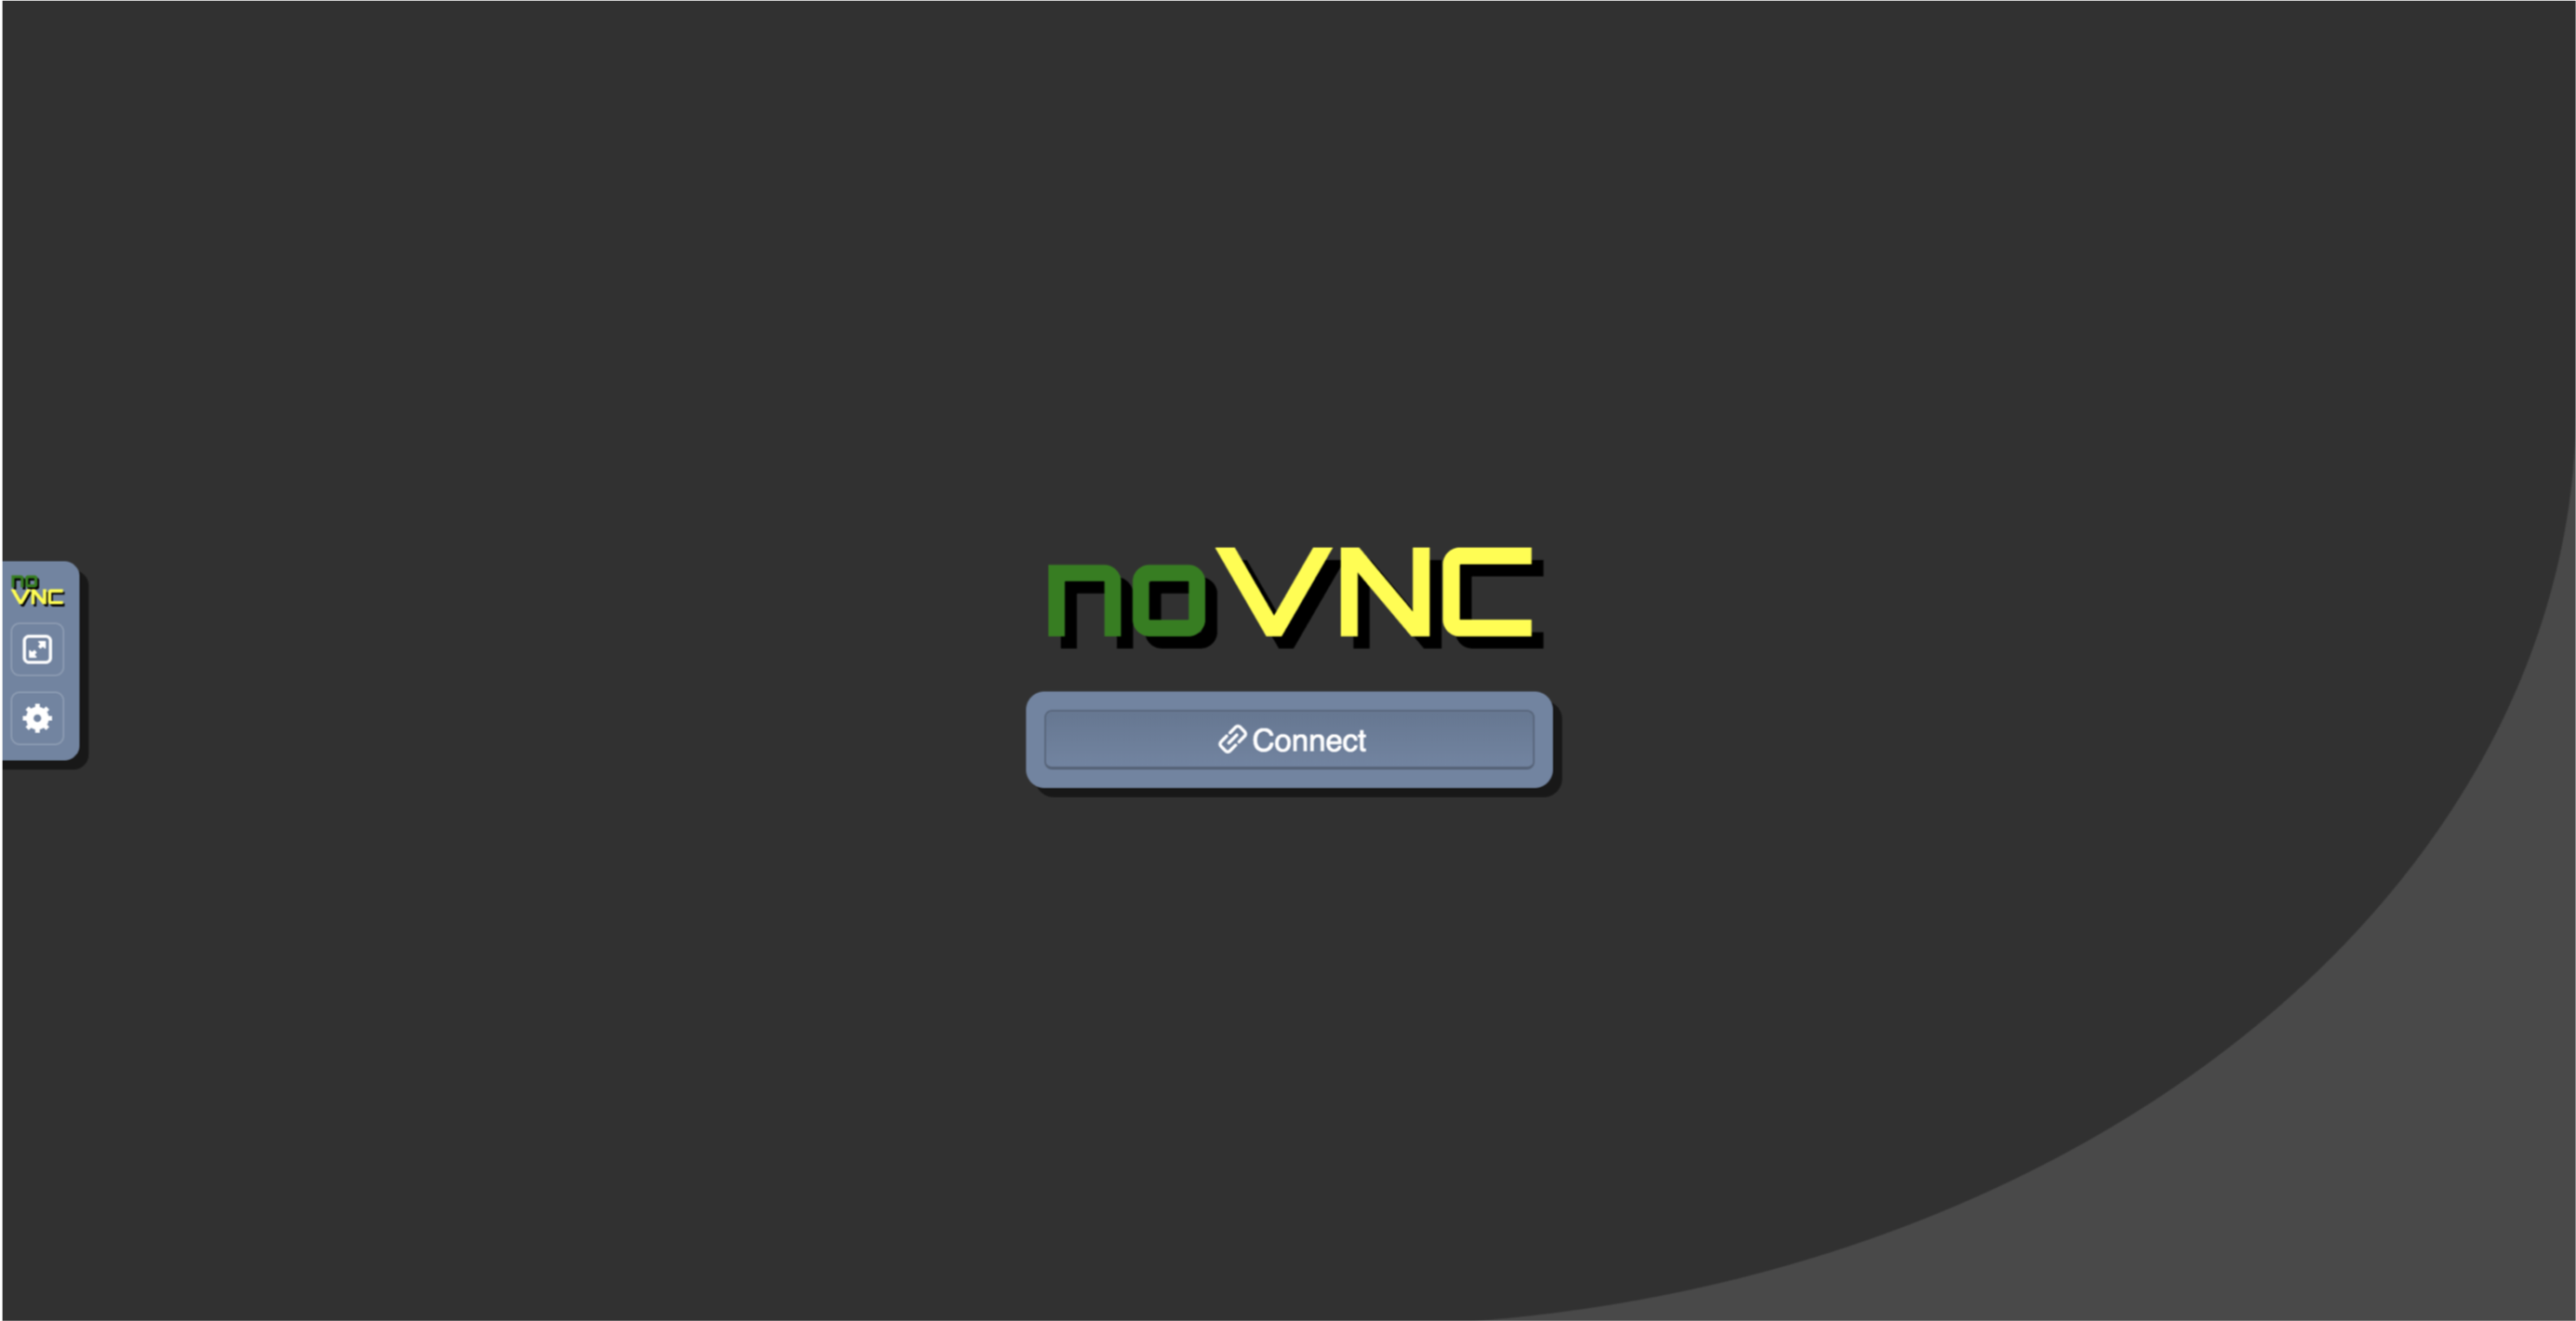
\includegraphics[scale=0.25]{docker.png}
\end{center}
Click connect and enter the super secret password: \textbf{cs2110rocks}

If you don’t want to use the browser, you can also connect using any VNC client. In order to connect, use the same base URL as the browser, but use the port \textbf{5901} with nothing after it.

That’s it! You should be up and running with what looks like a virtual machine running in your browser! If you open up the File Manager and look along the left, you should see a device called \textbf{host}. This is the folder that you had the \textit{cs2110docker.sh} script in. It has been mounted inside of the container. \textbf{When you are doing your work, you should edit all of you files in this folder ON YOUR HOST MACHINE. Then, use the Docker container to run the code. DO NOT EDIT FILES INSIDE THE CONTAINER. THEY WILL DISAPPEAR. PLEASE DON’T DO IT. PLEASE.} You will not get extensions on projects because you saved stuff where you should not have. We are making this very clear up front. Don’t do it.

When you are done using the container, you can shut it down by running

\begin{center}
    \begin{verbatim}
        ./cs2110docker.sh stop
    \end{verbatim}
\end{center}

If you are interested in running the container in the shell (no graphics), you can run

\begin{center}
    \begin{verbatim}
        ./cs2110docker.sh -it
    \end{verbatim}
\end{center}



\section{Wrap up}
That’s about all that there is to the CS 2110 Docker container setup. If you have any questions or issues, please post on Piazza \textbf{under the Docker folder}, so we can sort through Docker questions efficiently.

\section{Addendum: What even is Docker??}
I’m so glad you asked. In order to answer this question we have to go back in time.

\subsection{Physical Servers}
Back in the stone age, when application developers wanted to deploy their application, they first had to procure a server. These servers were very expensive, and for various reasons they could run a very small number of applications on each server. They also had to make sure their servers were powerful enough to handle a high load, so at times of lower load, there were a lot of wasted resources that were not doing anything. Monsters stalked the night, storms filled the skies, pestilence ran through the streets, and death was common. This obviously was a pretty big problem.

\subsection{Virtual Machines}
In order to help minimize the amount of resources that were wasted on servers, people started using ``Virtual Machines.'' Virtual machines are essentially computers within computers. First, you start with a physical server and install an operating system. On top of this operating system, you install something called a ``hypervisor.'' A hypervisor is a type of virtualization technology that allows us to emulate the hardware of a computer and install more operating systems on top of the main operating system. These guest operating systems are called virtual machines. With virtual machines, we can have one physical server and run multiple operating systems, which means that we can run multiple applications and thus not waste a ton of space. Problem solved! Here is a picture to illustrate how virtual machines work:
\begin{center}
    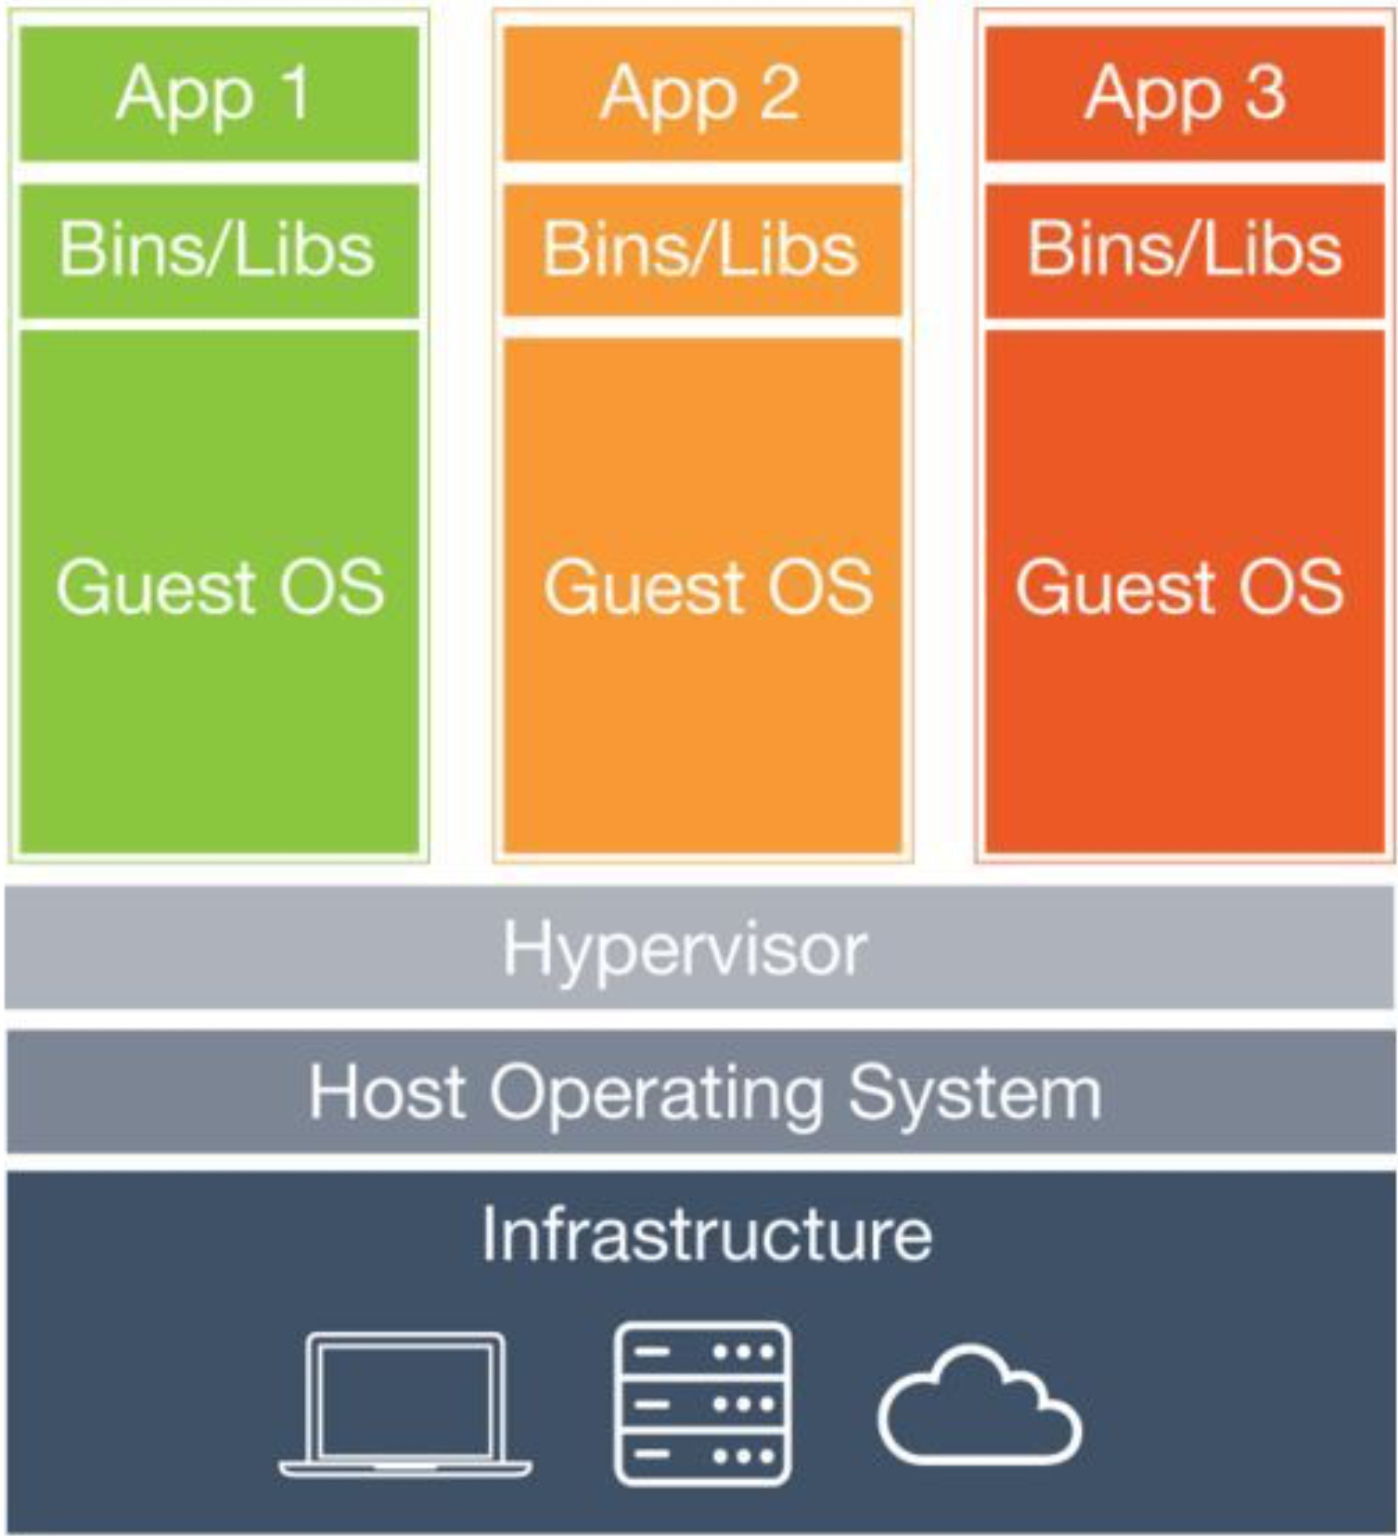
\includegraphics[scale=0.4]{virtualmachine1.png}
\end{center}

\subsection{What now?}
So we have fixed the problem of wasted resources. Time to kick back and put our feet up and be happy with everything we’ve accomplished, right? Well, if you take a look at the picture, guest operating systems are duplicated multiple times and taking up a bunch of space. Creating entire guest operating systems is incredibly wasteful. If you think about it, there is a ton of stuff that is duplicated. Each guest operating system has copies of the same base files and programs that make it up. In addition, emulating multiple operating systems takes a TON of system resources, which does not leave much for the applications themselves. So while we have solved the problem of having extra resources that are not utilized, we now have the opposite problem. We are using a ton of resources to do the exact same stuff multiple times. What if we could redirect these resources so that the applications themselves could have more to work with?

\subsection{Containers}
A few years after the concept of virtual machines was developed, some very smart people out there came up with the concept of ``containerization.'' Containerization is another type of virtualization, but instead of making multiple guest operating systems on top of an existing operating systems like virtual machines do, containerization divides the resources of the host operating system. Containerization involves creating ``containers,'' which are essentially sandboxes for applications to run in. By sandbox, I mean that it utilizes resources of the host operating system, but cannot impact anything outside of it. This provides a safe space for applications to run in. Each container gets its own chunk of everything that it could need from the host operating system---file system, system tools, network stack, etc.

\subsection{Docker}
Docker is an open source project that began in 2010 with the goal of providing abstraction to containers. Using Docker, application developers are able to quickly and easily containerize their applications. In order to use Docker, the host machine runs the Docker Engine, which handles the management and creation of containers. Here is a picture showing how containerization with Docker works (compare this to the Virtual Machine Picture):
\begin{center}
    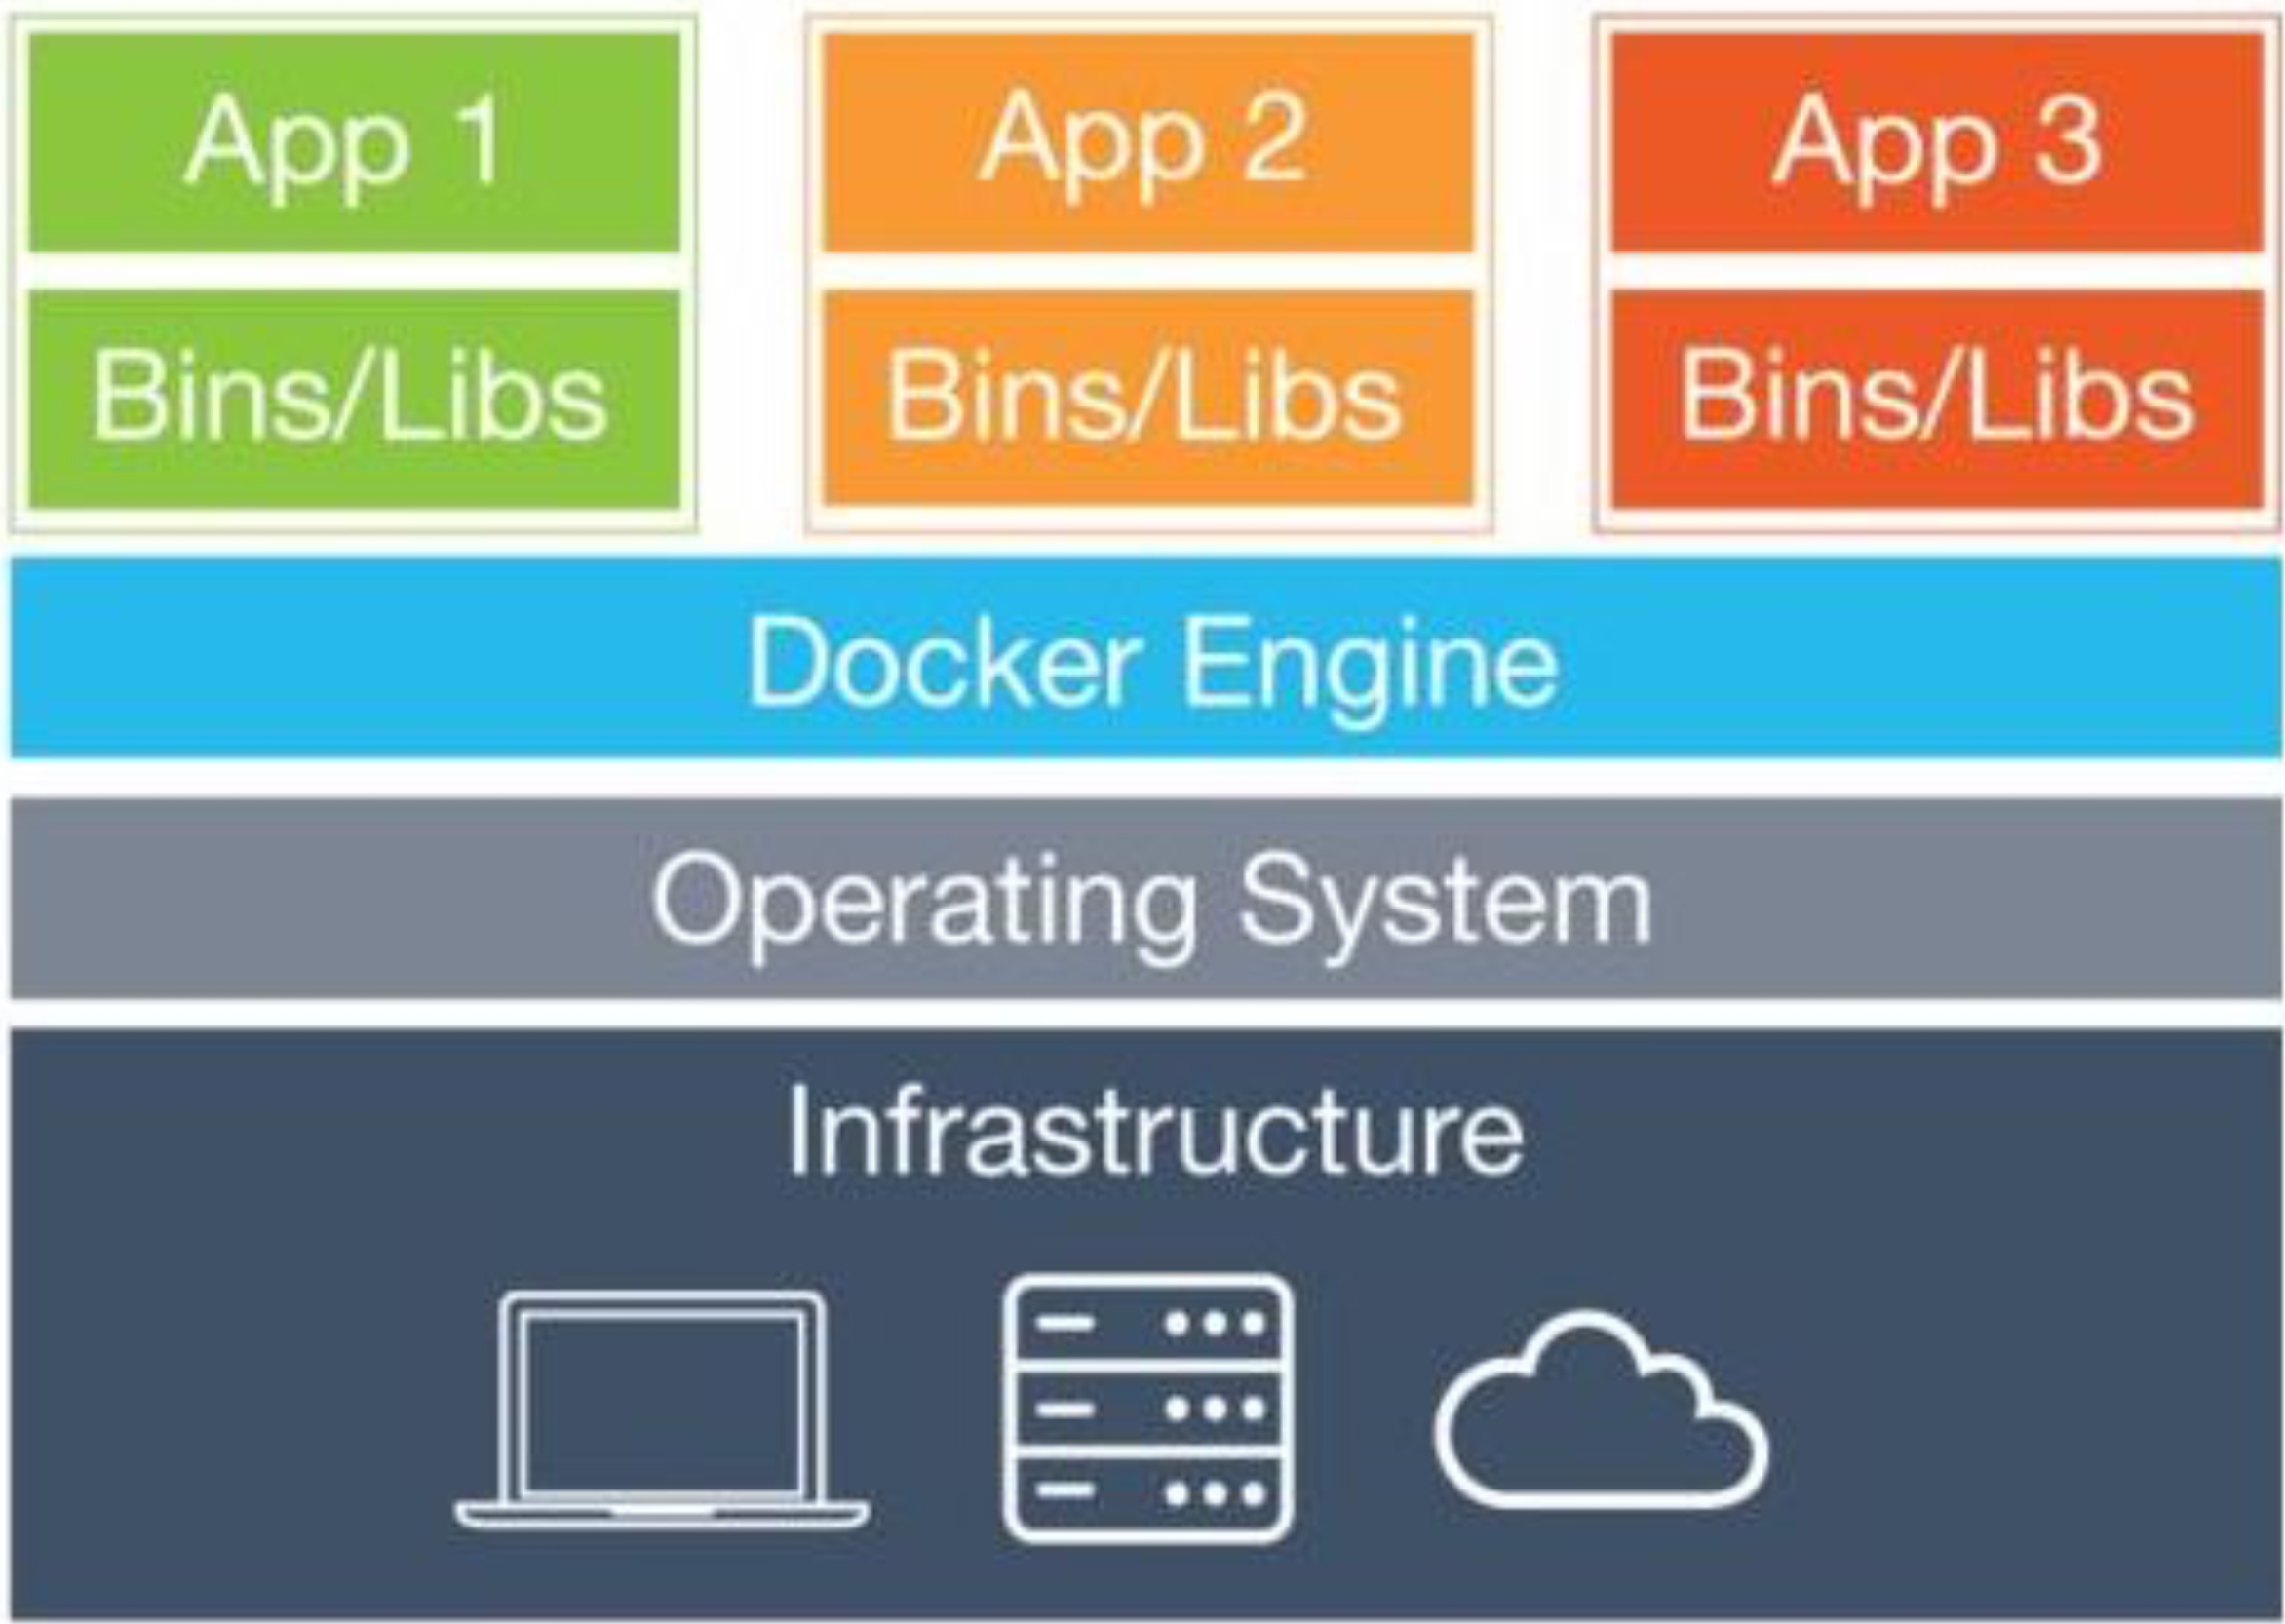
\includegraphics[scale=0.2]{virtualmachine2.png}
\end{center}
As you can see from the image, we no longer have to make multiple copies of the same operating system to run multiple applications. Instead, everything shares the resources of the host operating system.
Docker is designed to be run on Linux machines (since containers are dependent on the operating system they are running on), but they also provide solutions that will run on Windows and Linux using very very lightweight virtual machines.

\subsection{CONTAINERS ARE STATELESS}
There is one key component that we can not stress enough (and will continue to remind you of). Containers are stateless. They are designed so that they can be easily destroyed and recreated (which helps make them so lightweight). This means that any files saved inside a container or any changes made to it will be erased the second that the container is terminated. If you are working on something inside a container, you have to make sure you save it outside of the container before shutting the container down.





\section{Addendum: Why should I care about docker?}

Good question! Previously, we had our students install virtual machines in order to complete their assignments for this class. It worked fine for some, but many had at least one of the following issues:

\begin{itemize}
  \item VMs crashing all the time
  \item VMs not connecting to internet
  \item VMs running incredibly slow
  \item Issues installing tools that the class needs
  \item Random issues that only apply to a single student and can only be solved by deleting the VM and creating a new one (which takes forever)
  \item A ton more
\end{itemize}

As a result, we are using Docker to mimic a VM. This isn't precisely how Docker is meant to be used, but it will provide a lot of benefits including:

\begin{itemize}
  \item Serious performance improvements
  \item No networking issues because you won’t use the network with it
  \item Seamless integration with your host operating machine
  \item Comes pre-installed with all the tools that you will need
  \item The TAs can release updates/fixes mid-semester without any action on the students' part
  \item Since containers are stateless, if you have any problems, all you have to do is delete it and create a new one, which takes about 5 seconds
\end{itemize}

